\documentclass[tesis.tex]{subfiles}
\begin{document}
    
\section{Results}

The Pescadero Estuary, located at the confluence of Pescadero Creek and Butano Creek on the California coast, is a small and highly stratified estuary. It is characterized by an intermittently opening and closing inlet, where a sandbar acts as a barrier between the estuary and the sea. During the dry season, the sandbar closes the inlet, transforming the estuary into a stratified lagoon.\\

Field measurements were conducted between 17 Jan. 2012 and 21 Mar. 2012, capturing the estuary's conditions during this period. In Fig. \ref{fig:results} is shown the main data captured in the field campaign period. Fig. \ref{fig:results}A shows the density in the watercolumn with the water level, both in DC location. Fig. \ref{fig:results}B shows wind velocity in $u-v$ coordinates, where $v$ is the cross-estuary direction and $u$ is the along-estuary direction, in which offshore is positive and onshore is negative. Fig. \ref{fig:results}C shows tidal height in MLLW datum and significant wave height. Fig. \ref{fig:results}D shows the discharge of the Pescadero Creek. Tidal height, significant wave height and discharge are data external to the campaign. 

\begin{figure}[h!]
  \centering
  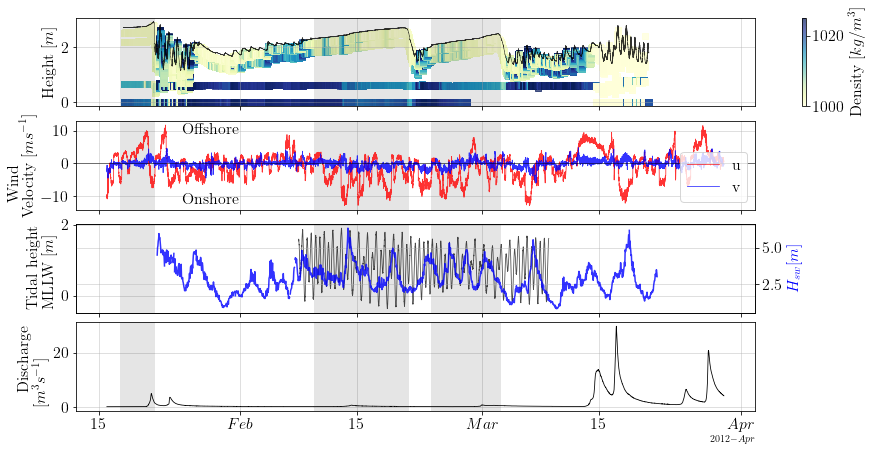
\includegraphics[width=\textwidth]{Imagenes/results.pdf}
  \caption{Time-series windowing the closed state of (A) colormap of density in DC location in the water column height, where the black line represents the water level; (B) wind speed in $u$ and $v$ direction; (C) tidal height in MLLW datum (black line) and significant wave height (blue line); (D) discharge.}
  \label{fig:results}
\end{figure}

 The inlet was initially closed when the sensors were installed and remained closed until 21 Jan. 2012. Subsequently, the inlet closed again on 07 Feb. 2012 and reopened on 21 Feb. The estuary experienced its third closure on 24 Feb., which persisted until 3 Mar. (Fig. \ref{fig:results}A).\\
 
 When the mouth closes in Pescadero we can observe that the flow of water between the estuary and the sea is significantly reduced, almost completely blocked, event that is presented as a decrease of density at surface and a stabilization of estuarine height (Fig. \ref{fig:results}A). This restricted exchange isolates the estuary from the influence of oceanic processes and creates a more confined waterbody. One consequence of the inlet closure is the establishment of stratification within the estuary. In Fig. \ref{fig:results}A we can observe lighter freshwater sitting atop denser saltwater.\\

 Wind speed is higher during the closed state periods (Fig. \ref{fig:results}B), not necessarily due to any important factor in our study, but it does influence how the estuary behaves in the closed state. The tidal behavior looks normal as does the significant wave height (Fig. \ref{fig:results}C). Fig. \ref{fig:results}D shows that discharge can change the estuary behavior (Fig. \ref{fig:results}A), as on 21 Jan., a slight increase in discharge helped to increase the water level, and then opening the sand bar. Small increases in flow are observed on 14 Feb. and 1 Mar., which are not as significant but may affect when the swell is restricted.\\

\subsection{Conditions observed during the closed state}

Abrupt decreases in water level that were proceeded by a slow increase in the estuarine water level without tidal influence were identified as mouth openings and when tidal energy is not visible at the water level there is a mouth closure. We observed that the inlet opened three times and in each one there are abrupt density changes in the water column along with other important conditions that we are going to address below.

\subsubsection{Wind in the estuary}

In Fig. \ref{fig:windrose} we can observe that the wind is mainly bidirectional and when it goes onshore the magnitude is bigger. Directions between 300 and 360 degrees come from the ocean and the wind that blows from 100 to 170 degrees comes from inland. This form is due to the topography of Pescadero which has an escarpment at the south of the inlet, protecting the mouth. Also, the marsh itself is located in a low valley, constricting wind flow paths. For the along-estuary velocity, ($u$) we observe that the maximum velocities reach between 10 and -10 m/s approximately (Fig. \ref{fig:windvel}). In the cross-estuary velocity, ($v$) we observed just a few spikes where the maximum velocity was reached, at approximately 5 and -5 m/s. 

\begin{figure}[h!]
    \centering
    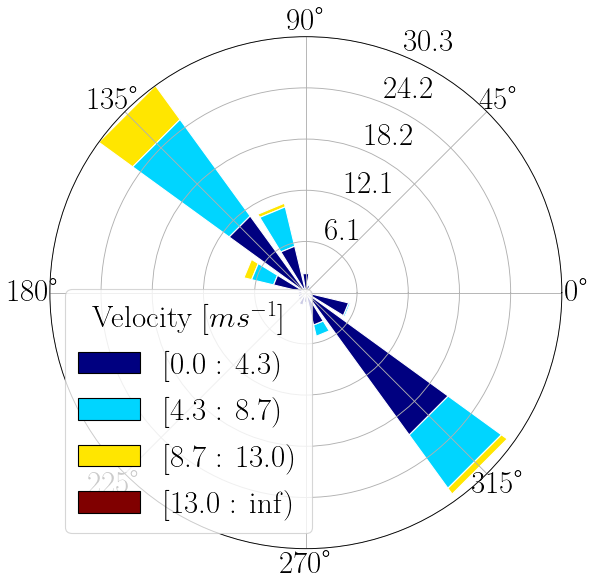
\includegraphics[scale=0.3]{Imagenes/windrose.png}
    \caption{Windrose of the data collected in Pescadero from 15 Jan. to 20 Mar. Maximun speed registered in the studied period was 13.02 m/s}
    \label{fig:windrose}
\end{figure}

\begin{figure}[h!]
  \centering
  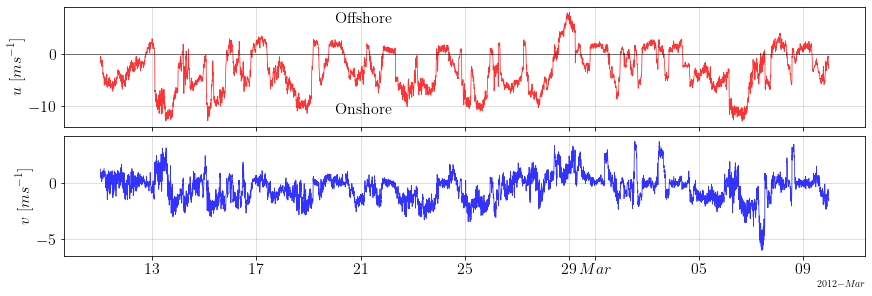
\includegraphics[width=\textwidth]{Imagenes/wind_vel.png}
  \caption{Time-series of wind speed in $u$ and $v$ direction (see Fig. \ref{fig:wind_raw}).}
  \label{fig:windvel}
\end{figure}

\subsubsection{Evolution of density structure}

 Pescadero estuary is characterized by having a strong thermohaline stratification in its closed state. Fig. \ref{fig:saltemp} shows the temperature (Fig. \ref{fig:saltemp}A), salinity (Fig. \ref{fig:saltemp}B), density with height above the bed (Fig. \ref{fig:saltemp}C) and the change of water level in time (Fig. \ref{fig:saltemp}D).
 
 When the estuary inlet starts closing, temperature and salinity acquire different values on the top and bottom of the lagoon, increasing density change in the vertical \citep{largier2015}. The sand bar that forms at the inlet of the estuary contains the freshwater inflow and does not allow the waves to enter, but during high tide the waves could be overtopping it \citep{laudier2011measured}, contributing to the salinity in the system. This, depending on the magnitude of the intrusion, could affect the stratification of the entire estuary.\\

\begin{figure}[h!]
    \centering
    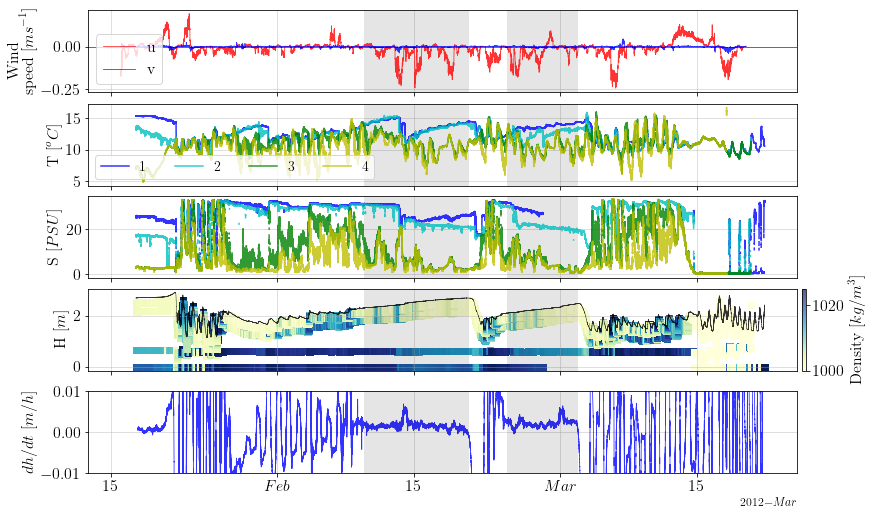
\includegraphics[width=\textwidth]{Imagenes/saltemp.pdf}
    \caption{Time-series windowing closed state of (A) temperature and (B) salinity in NM, where 1 is the deepest sensor and 4 the shallowest; (C) colormap of density in NM with height above bed, showing the position of each sensor, where the black line represents the water level, and (D) the change of the water level in a 10-hour frame.}
    \label{fig:saltemp}
\end{figure}

\begin{figure}[h!]
  \centering
  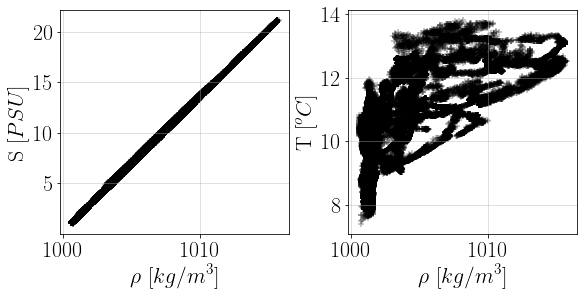
\includegraphics[scale=0.5]{Imagenes/salT_dens.png}
  \caption{Salinity and temperature versus density}
  \label{fig:saltdens}
\end{figure}

We defined the closed state at the estuary when the depth's change in time $\Delta h/\Delta t$, with $\Delta t=10$ hours, is positive and less than 0.01 m/h for more than a day (Fig. \ref{fig:saltemp}), meaning that the lagoon is filling with fresh water, increasing its level, and with a low influence from the sea. In that context Pescadero is in closed state three times: in mid January, in mid February, and in late February/early March where the first one is at the start of the time series, not including the initial closure, while the second and third closures are in gray shadow (Fig. \ref{fig:saltemp}). The differences between these three closures are that the first has the highest water level, and the second and third closures never get to the same level. \\

It is known that the first breach of the bar was artificial \citep{Williams2014}, openings that according to \cite{Behrens2013} would be less effective in keeping the mouth open than those that developed naturally, as in this case when the estuary is in an open state for just a couple days. The second barrier breach is believed to have occurred naturally. \\

In the time series, we observed during the closed state the temperature and salinity went stratified (Fig. \ref{fig:saltemp}). We observed a lower and non-stable temperature at the surface (Sensors 3 and 4 in Fig. \ref{fig:saltemp}) due to the cold season and the following day-night temperature changes. The temperature at the bottom (Sensors 1 and 2 in Fig. \ref{fig:saltemp}) is more stable, but still being influenced by daily changes and other external factors, indicating for example an abrupt fall on 13 Feb., followed by another increase. The bottom salinity is also steady most of the time and is generally decreasing. The surface salinity is more vulnerable to external factors and only is more stable during the closed state. \\ 

During the closed state, we observed three layers in the density structure with the superior one getting thicker upstream. In Fig. \ref{fig:perfiles1} there is the longitudinal view of the estuary densities from the profiles and the moorings. The moment the profiles were made (16 Feb. at 5 pm, see Fig. \ref{fig:windvel}) the wind was calm, so is not causing a disturbance in the water. We can observe that near the mouth the salinity is higher or the water column is more homogeneous. After a few days in a closed state, the estuary opened on 12 Feb. and 3 Mar. observing a decrease in water level (Fig. \ref{fig:saltemp}). \\

\begin{figure}[h!]
    \centering
    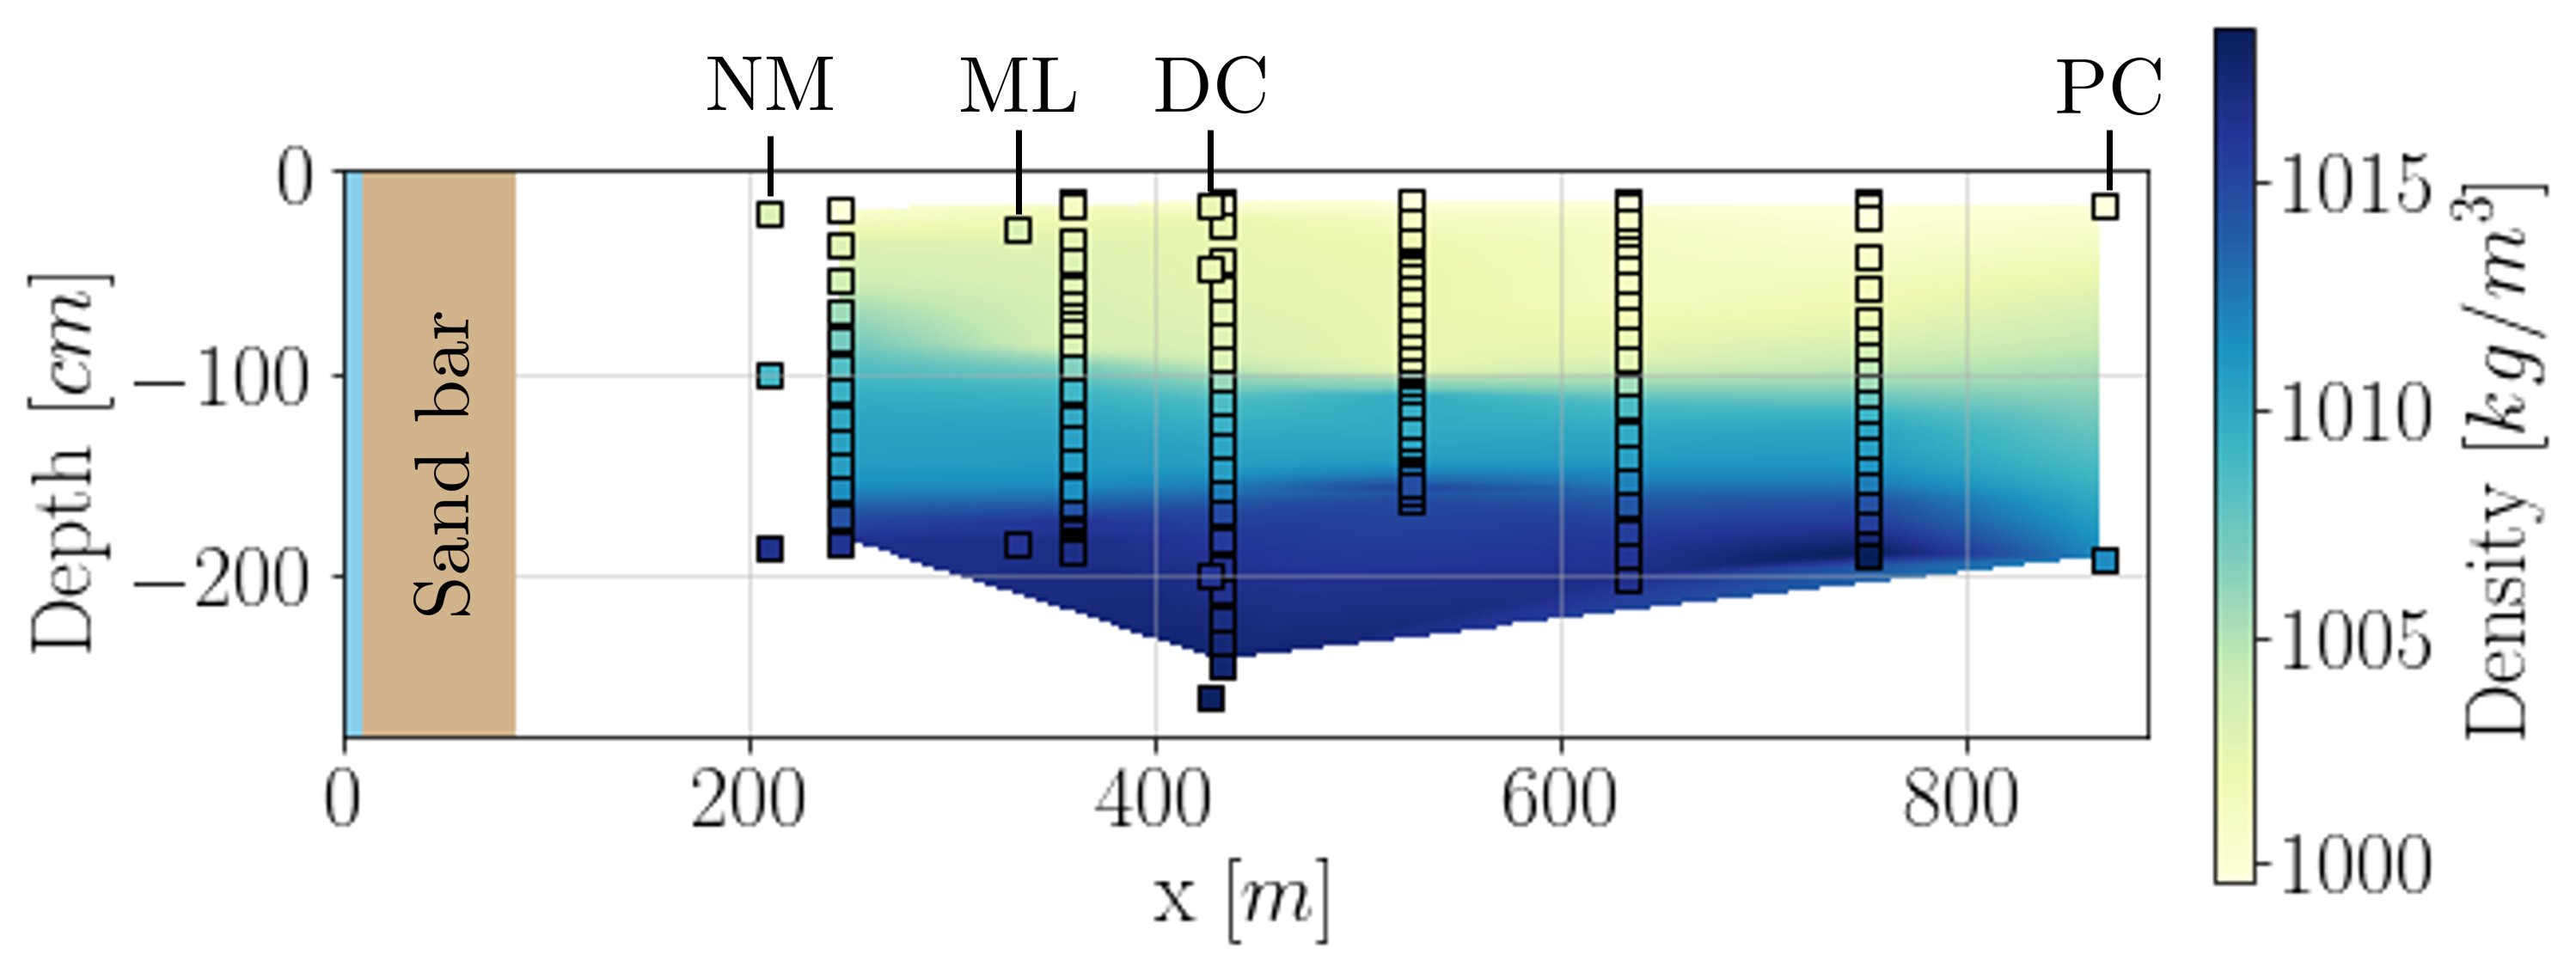
\includegraphics[scale=0.6]{Imagenes/vista_long2.png}
    \caption{Along-estuary density colormap of Pescadero. Distance x is considered from the coast following the curvature of the estuary as the sensors are placed in Fig. \ref{fig:mapPDO}. }
    \label{fig:perfiles1}
\end{figure}

\subsubsection{Tidal and waves conditions}

In Fig. \ref{fig:wave1} we have the wave conditions for Pescadero during the study period. We can observe, that when the mouth is open tidal influence is present in Pescadero, but when the mouth closes we cannot observe an evident effect in plain sight, which does not mean there is not present. Significant wave height goes from 2.5 m to more than 5 m approximately, but we have to account that deep water wave heights are larger than wave heights experienced at the coast \citep{Williams2014}, and as this data where collected 40 km from shore, thus we use this value as a proxy for coastal ocean conditions.  \\

The rest of the parameters (wave periods and direction) were collected from the same buoy, so they also are an approximation of the wave conditions. Dominant periods go from 5 to 20 s, while averaged periods have a range only between 7 and 10 s. The direction of the dominant period is stable at around 300 degrees most of the time, with just a peak on 29 Feb. where reaches 250 degrees.\\

\begin{figure}[h!]
    \centering
    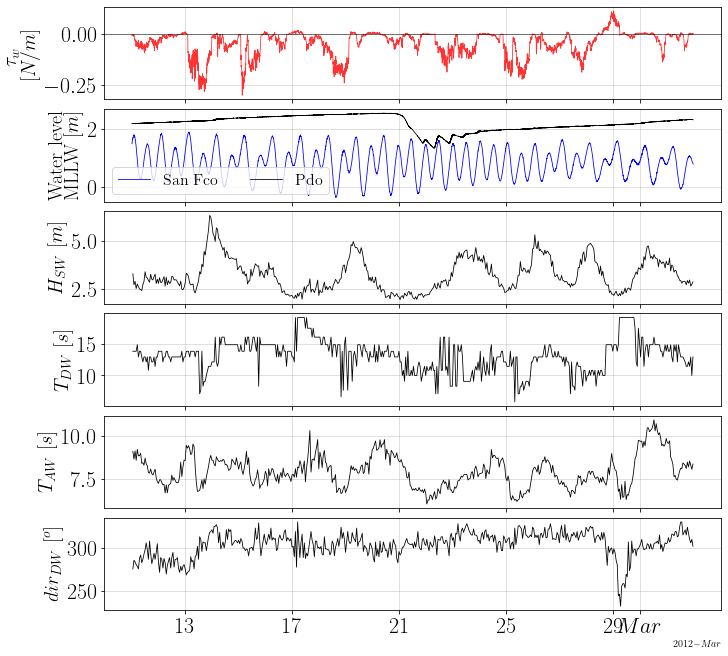
\includegraphics[width=\textwidth]{Imagenes/wave1.png}
    \caption{Time-series of tidal height in San Francisco (blue) and Pescadero estuary water level (black) in MLLW datum, significant wave height ($H_{SW}$), dominant wave period ($T_{DW}$), average wave period ($T_{AW}$), and the direction from which the waves at the dominant period are coming ($dir_{DW}$).}
    \label{fig:wave1}
\end{figure}

\subsubsection{Pescadero creek discharge}

Pescadero estuary receives freshwater from Butano Creek and Pescadero Creek, where the latter is the one that contributes the most to the lagoon and the one we have available data. When the inlet is closed, the maximum flow recorded was $0.72$ $m^3/s$, lower than the usual for winters in California, presenting two small increases in flow (Fig. \ref{fig:q}), but which, due to their low magnitude, would not be a determining factor in the rupture, considering that between July 2011 and July 2012 the maximum flow was $29.73$ $m^3/s$. Even so, there is a constant inflow of fresh water that increase the estuary water level progressively until the inlet breaks.  

\begin{figure}[h!]
    \centering
    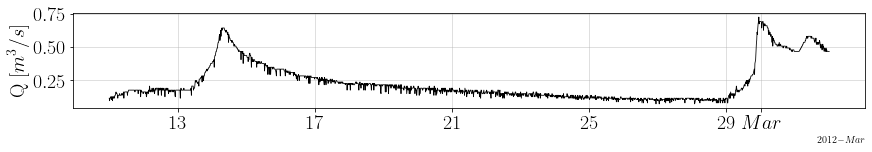
\includegraphics[width=\textwidth]{Imagenes/Q.png}
    \caption{Time-series of freshwater flow from Pescadero Creek.}
    \label{fig:q}
\end{figure}

\subsubsection{Currents speed and direction}

During the closed state, the wind direction is predominantly onshore and its magnitude in that direction is bigger than in the rest of the period (See Fig. \ref{fig:windvel}). Surface wind stress over the closed estuary causes the upper layer to go in the same direction as the wind, and the lower layer to move in the opposite direction \citep{Katopodes2018}. Given the limitations of the ADCP sensor, velocities near the surface were not always captured, therefore, there is a range of speed observable, not showing what happens at the bottom or the surface. Pescadero has its main directions very marked, a case that is very particular in this kind of estuaries, where along-estuary velocities always domain the currents. \\

\subsubsection{Surface fluctuations}

We can observe, that when the mouth is open tidal influence is present in Pescadero's water level, and when significant wave height increases the influence is also larger (Fig. \ref{fig:wave1}). When the bar blocks the inlet, this causes accumulation of the upstream freshwater in the lagoon which is represented as an increase in Pescadero's water level. The closure reduces the ocean influence to be negligible to plain sight, but still could be wave overtopping the inlet sandbar. These wave overtopping events could be detected by the fluctuations in the surface present in the data, but also we have to consider the fluctuations caused by wind stress or by an increment of the discharge.\\

\subsection{Hydrodynamic controllers}

The external factors that could be affecting the estuary in a closed state are freshwater inflow, saltwater overtopping from waves, and wind stress. There are other factors involved as temperature or evaporation, but we estimated that those were negligible due to the haline stratification that dominates the estuarine structure.\\

\subsubsection{Stratification controllers}

At the beginning of both periods of disconnection, we noticed that there were changes in densities on the surface and in the deep layer, although the latter in smaller magnitude and fewer times (Fig. \ref{fig:dens}). Three important wind events occurred in each period that matches with the increase in surface densities, observing that when the stress on the surface increases, so does the density in the upper layer in the three sites. When wind forcing decreases, we noticed that density tends to return to its initial state, except for the largest events at the beginning of each period, where density at the bottom is smaller after the event than before.\\

\begin{figure}[h!]
    \centering
    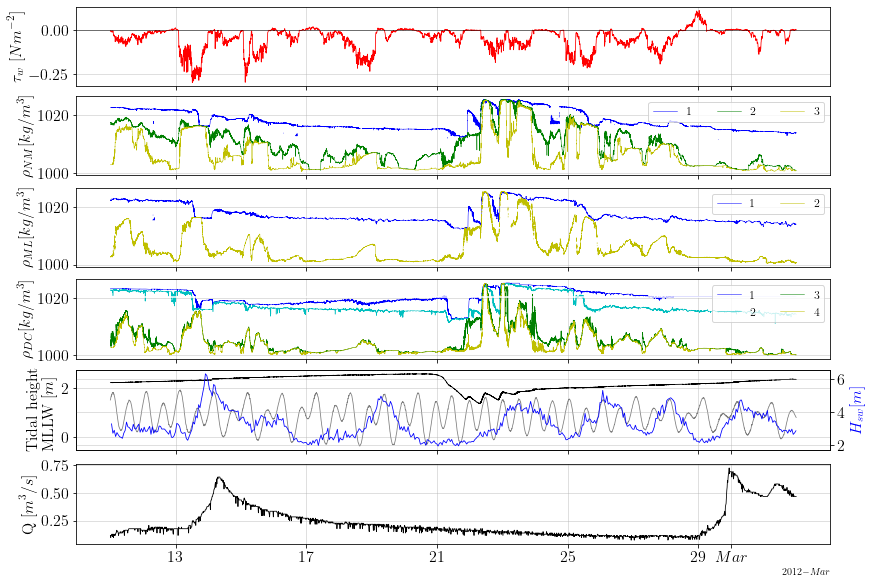
\includegraphics[width=\textwidth]{Imagenes/dens.png}
    \caption{Time-series of wind stress ($\tau_w$), NM ($\rho_{NM}$), ML ($\rho_{ML}$), and DC ($\rho_{ML}$) densities in different depths, where sensor 1 is the deepest and sensor 4 is the shallowest (The positions in the water column of the sensors are shown in Fig. \ref{fig:perfiles1}), significant wave height in Halfmoon Bay in blue ($H_{sw}$), Pescadero estuary water level (black) and tidal height in San Francisco (gray) in MLLW datum, and freshwater inflow of Pescadero creek ($Q$).}
    \label{fig:dens}
\end{figure}


Upstream inflow had two increasing events in the studied period (Fig. \ref{fig:dens}) and during those events, there wasn't an instant change in density, but we could notice a trend in density, especially in the lower layers, which was decreasing in time during both disconnected periods on NM and ML sites. In the first period, at the DC location, unlike the others, there was an increasing trend of density, which would not be unusual considering the lower layer of DC is much deeper than the ones of NM and ML (Fig. \ref{fig:perfiles1}), furthermore, the layer in DC with the same depth to those is the one before the deeper (in cyan, Fig. \ref{fig:dens}). Another change in density that is noticeable occurs in the middle layer of NM (in green, Fig. \ref{fig:dens}) between 13 Feb. and 17 Feb., just before and after there was an increase in discharge. There we observed that density went from around 1015 $kg/m^3$ to almost 1000 $kg/m^3$. \\

Significant wave height and tidal height could be showing some wave overtopping events when there is high tide and high waves, but this does not mean there couldn't be wave overtopping when there is only high tide. Even though we do not observe important increases in density that indicate an important saltwater input, so we cannot know when happens. Anyways, there are small changes in density both on the bottom and on the surface.\\

First, we observed density fluctuations at the surface but without causing important changes on 14 Feb., 16 Feb., 19 Feb., 20 Feb., 26 Feb., 27 Feb., and 1 Mar, while there was high tide and sometimes high waves, but all of them happened right after a wind event or during an increase of discharge (Fig. \ref{fig:dens}), so we can't assume that one factor or another is causing it. Second, at the bottom, we observed some density increases that were momentary on 15 Feb., 26 Feb., 27 Feb. and 28 Feb. during high tide, and mainly noticeable in NM, which is the closest site to the sea. Those increases do not look like the increases in salinity caused by wind effects, because the salinity is bigger than before the wind event in some cases, although, as this still happens when there was a wind event we can't attribute it just to wave overtopping. Third, there was a continuous increase in DC at the bottom that happened after an important decrease in salinity due to a wind event.\\

\subsubsection{Surface fluctuations controllers}

If we focus on the depth at Pescadero we can observe more clearly how external factors are changing the estuary. The wavelet frequency analysis of depth can show the effects of the waves into the lagoon, by identifying changes in its fluctuations and showing when there is the presence of certain frequencies that could represent the ocean influence. If we crossed this information with tidal behavior and significant wave height we can obtain a more certain way to identify wave overtopping events. \\

We notice that when the estuary is open the ocean effects are very marked in the wavelet analysis (Fig. \ref{fig:surf}). During a closed state, the effects are also evident but more slightly, with more concentrations of frequencies between 0.02 and 0.1 Hz, and we could point out that those are wave overtopping events. Also, we can say that they occur exclusively at high tide, and any wave height, but the events are bigger when the waves are larger. On the other hand, wave overtopping does not have a clear pattern of behavior in $dh/dt$ or $(\hat{H}_{DC}-\hat{H}_{ML})/\Delta x$ when the inlet is closed.\\

\begin{figure}[h!]
    \centering
    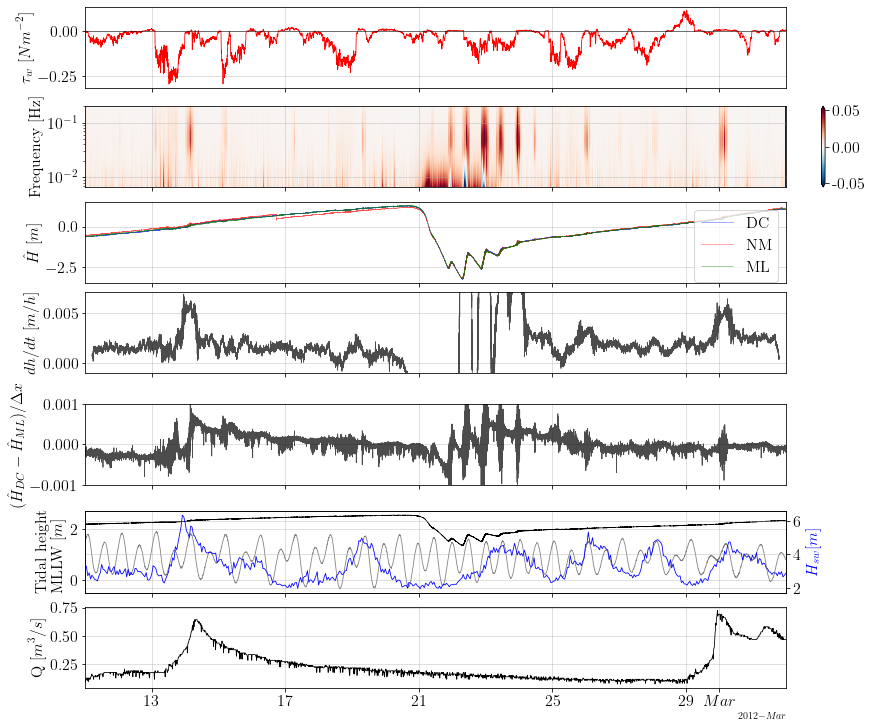
\includegraphics[width=\textwidth]{Imagenes/surf.png}
    \caption{Time-series of wind stress ($\tau_w$), depth wavelet frequency analysis at DC, standardized depth ($\hat{H}$) in DC, NM, and ML locations, the change of the water level in a 10-hour frame ($dh/dt$), standardized depth change between locations DC and ML ($(\hat{H}_{DC}-\hat{H}_{ML})/\Delta x$), significant wave height in Halfmoon Bay (blue), Pescadero estuary water level (black) and tidal height in San Francisco (gray) in MLLW datum, and freshwater inflow of Pescadero creek ($Q$).}
    \label{fig:surf}
\end{figure}

As we notice earlier, the discharge has two increase events during the studied period. We can observe that those increases are affecting directly the surface, showing important peaks of $dh/dt$ during those events (Fig. \ref{fig:surf}). Also, the change of the standardized height in the horizontal ($\Delta \hat{H}/\Delta x$) showed at the beginning of the period negative values which changed to positive values after the increase of discharge, which also results in happens after a strong wind event and during a wave overtopping.\\

\subsection{Wind-driven effects}

As mentioned before, we noticed changes in density at the same time there were wind events, therefore for quantifying those changes we calculated the potential energy anomaly of the water column in location NM and compared it to wind stress (Fig. \ref{fig:phi}), where we noticed that there were a lot of similarities between both time-series. We observed that when wind stress magnitude increases, potential energy anomaly decreases, except when there are positive values like on 28 Feb. and 29 Feb, when there was no change in potential energy anomaly. However, we can notice that the potential energy anomaly has not the same behavior in wind events of the same magnitude, and we can observe that, in time, wind decreases its effect on the potential energy anomaly, only reaching 0 at the first wind event of each period. In addition, we can observe that after those events there is a decrease in potential energy anomaly when wind stress is zero, probably showing a change in their stratification structure after those events.\\

\begin{figure}[h!]
    \centering
    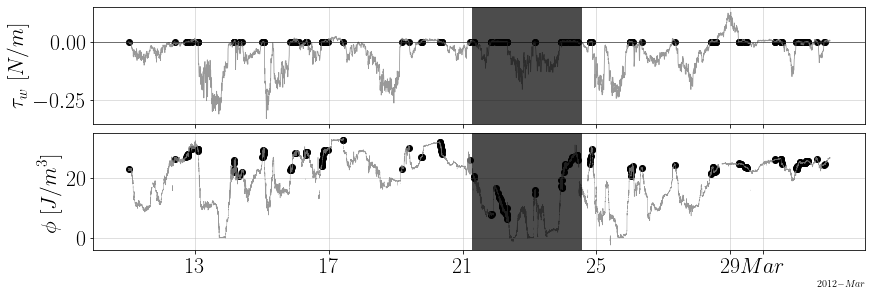
\includegraphics[width=\textwidth]{Imagenes/phi.png}
    \caption{Time-series of wind stress ($\tau_w$), and potential energy anomaly ($\phi$). Dots are the instant when wind stress is zero. The shadowed window is when the estuary is in an open state.}
    \label{fig:phi}
\end{figure}

For further understanding, we implemented the Wedderburn number to observe if there was upwelling due to wind events. As we did not have the thickness of the epilimnion we estimated a range of positions for the pycnocline. This range started right after the first CTD, the deeper one (in black), and ended in the second CTD (in grey) (Fig. \ref{fig:wedd}). Also, we marked with a star where was the epilimnion limit on 16 Feb., when we had more information on the density (Fig. \ref{fig:perfiles1}), which could be changing in time. As we are working with a range of values, we considered a partial upwelling when just the upper boundary reaches W=1 and full upwelling when both boundaries reach that value. In each period we noticed one full upwelling event and two partial upwelling events, for a total of six upwelling events observed in the studied period, always the first one being fully upwelled (Fig. \ref{fig:wedd}). After full upwelling events, density at the bottom of the water column did not come back to its original values from before the event. \\

\begin{figure}[h!]
    \centering
    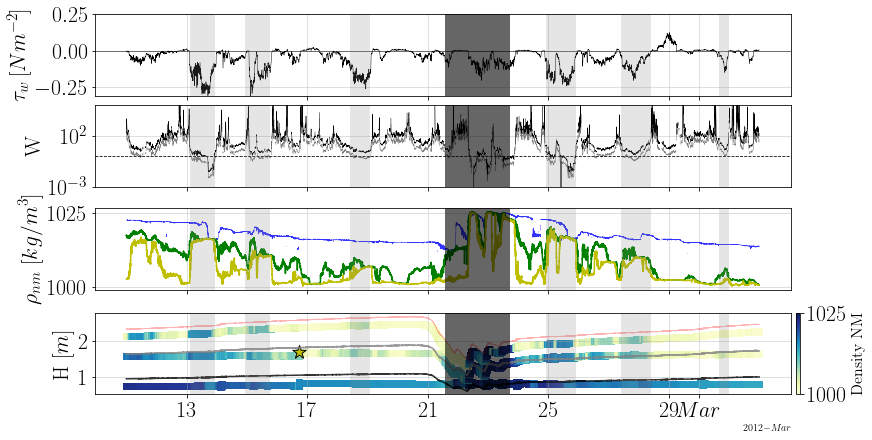
\includegraphics[width=\textwidth]{Imagenes/wedd.png}
    \caption{Time-series of wind surface shear stress ($\tau_w$), Wedderburn number ($W$) where the dashed line shows W=1 and black and gray lines show W obtained at the lower and upper part of the selected window respectively, density at the bottom (blue), middle (green), and top (yellow) of the water column in NM location ($\rho_{nm}$) (see Fig. \ref{fig:perfiles1} for sensors positions), and colormap of density in time-space at each sensor of location NM with the black and gray line that limit the lower and upper part of the window of possible values for top layer width. The dark shadowed window is when the estuary is in the open state. Light-shadowed windows are when the upwelling events were observed. Redline is the water level, and the star indicates where the surface layer ends according to Fig. \ref{fig:perfiles1}.}
    \label{fig:wedd}
\end{figure}

In Fig. \ref{fig:diff} we can observe how density at the surface is getting more resilient to wind effects over time. The three wind events in the first period are similar in magnitude, but the increase in density that they trigger is each time smaller. What's more, we can notice a small wind stress event at the beginning of the time series that increased density three times more than the last wind event in the period. We can also notice that density changes in the vertical ($\Delta \rho/\Delta z$) reached 0 at the first wind event of each period, but then, after the event, $\Delta \rho/\Delta z$ went steadier and didn't reach 0 again during the period.\\

\begin{figure}[h!]
    \centering
    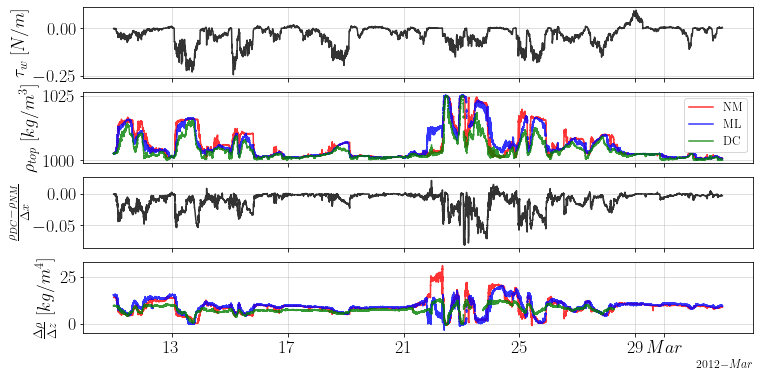
\includegraphics[width=\textwidth]{Imagenes/diff.png}
    \caption{Time-series of wind shear stress at the surface ($\tau_w$), surface densities in locations NM, ML, and DC ($\rho_{top}$), density change between locations DC and NM at the surface ($\frac{\rho_{DC}-\rho_{NM}}{\Delta x}$), and density change between surface and bottom in locations NM, ML, and DC ($\frac{\Delta \rho}{\Delta z} \; [kg/m^4]$).}
    \label{fig:diff}
\end{figure}

The first important wind event started on 13 Feb. at 2 a.m. and the first location that was affected was NM, then ML, and finally DC. We can prove the latter with the change of density along the estuary (Fig. \ref{fig:diff}) where we observed negative values almost all the time, showing higher values in NM than in DC. When the wind starts to blow there is an increase in $\Delta \rho/\Delta x$ magnitude, and after reaching the peak the value decreases again to zero and stays there if the wind speed is constant. If wind speed decreases there is another increase in $\Delta \rho/\Delta x$ magnitude, showing that the wind stops influencing DC location first and then NM.\\

To quantify the time difference between the moment the wind started blowing and the density started changing at the different CTD locations, we calculate by visual inspection how long it took for the wind to affect density at different points. To achieve this, we considered the moment that density just started to change into a trend after the wind started or stopped blowing. Also, to compare the obtained values we calculated the cross-correlation, between density and wind stress, after normalizing and standardizing both signals. We obtained the values of the first wind event, and how long took to start and finish, and for the cross-correlation, we added the total of the first-period lag.\\

In Table \ref{tab:lag} we observed that surface sensors (NM3, DC4, and ML2) had no delay with the cross-correlation method and did have it in the visual inspection. Also, with the latter method, we observed that NM3 was the last sensor that started to change after wind stress started, but it increased faster than the others, a fact that we can observe slightly in Fig. \ref{fig:diff} for $\rho_{top}$. Also, we observed that the one that took longer to come back to its initial value was NM3, then ML2 and DC4.\\

\begin{table}[]
    \centering
    \caption{Lag obtained by cross-correlation method and visual inspection. "Start" columns mean that lag was calculated only when the wind stress magnitude was increasing at the first event, and "end" columns mean that lag was obtained when the wind stress magnitude was decreasing at the first event.}
    \begin{tabular}{|c|cccc|ccc|}
    \hline
    Method &
      \multicolumn{4}{c|}{Cross-correlation} &
      \multicolumn{3}{c|}{Visual inspection} \\ \hline
    Sensor &
      \multicolumn{1}{c|}{Start} &
      \multicolumn{1}{c|}{End} &
      \multicolumn{1}{c|}{Total event} &
      Total period &
      \multicolumn{1}{c|}{Start} &
      \multicolumn{1}{c|}{End} &
      Total event \\ \hline
    NM1 &
      \multicolumn{1}{c|}{252 min} &
      \multicolumn{1}{c|}{132 min} &
      \multicolumn{1}{c|}{354 min} &
      384 min &
      \multicolumn{1}{c|}{810 min} &
      \multicolumn{1}{c|}{420 min} &
      615 min \\ \hline
    NM3 &
      \multicolumn{1}{c|}{0 min} &
      \multicolumn{1}{c|}{0 min} &
      \multicolumn{1}{c|}{0 min} &
      36 min &
      \multicolumn{1}{c|}{30 min} &
      \multicolumn{1}{c|}{225 min} &
      127 min \\ \hline
    DC1 &
      \multicolumn{1}{c|}{36 min} &
      \multicolumn{1}{c|}{0 min} &
      \multicolumn{1}{c|}{258 min} &
      732 min &
      \multicolumn{1}{c|}{630 min} &
      \multicolumn{1}{c|}{30 min} &
      330 min \\ \hline
    DC4 &
      \multicolumn{1}{c|}{0 min} &
      \multicolumn{1}{c|}{0 min} &
      \multicolumn{1}{c|}{0 min} &
      30 min &
      \multicolumn{1}{c|}{10 min} &
      \multicolumn{1}{c|}{0 min} &
      5 min \\ \hline
    ML1 &
      \multicolumn{1}{c|}{54 min} &
      \multicolumn{1}{c|}{174 min} &
      \multicolumn{1}{c|}{450 min} &
      600 min &
      \multicolumn{1}{c|}{615 min} &
      \multicolumn{1}{c|}{500 min} &
      557 min \\ \hline
    ML2 &
      \multicolumn{1}{c|}{0 min} &
      \multicolumn{1}{c|}{0 min} &
      \multicolumn{1}{c|}{0 min} &
      24 min &
      \multicolumn{1}{c|}{0 min} &
      \multicolumn{1}{c|}{55 min} &
      27 min \\ \hline
    \end{tabular}
    \label{tab:lag}
    \end{table}

    If we compared Table \ref{tab:lag} values to the response tilt time, obtained as the fourth part of the internal wave period, that is $11.75 \pm 2.72$ min, we observe that it is the most approximate to the values of the total period obtained by cross-correlation at the surface, but they are the double of it. Also, at the beginning of the event by visual inspection DC4 takes 10 minutes to start changing which, considering that DC is at the center of the estuary, could be the correct value.\\

    Surface wind stress over the closed estuary causes the upper layer to go in the same direction as the wind, and the lower layer to move in the opposite direction \citep{Katopodes2018}. Given the limitations of the ADCP sensor, velocities near the surface were not always captured, therefore, we observed a range of speed, not showing what happens at the bottom or the surface. On the other hand, Fig. \ref{fig:vels} shows that the along-estuary speeds ($u$) increase in proportion to the wind stress, but in opposite direction. The wind is also influencing cross-estuary velocity ($v$), but with less intensity due to the wind's main velocities. Vertical velocity ($w$) presents fluctuations and some negative or positive peaks during wind events or after in some cases. \\

    \begin{figure}[h!]
        \centering
        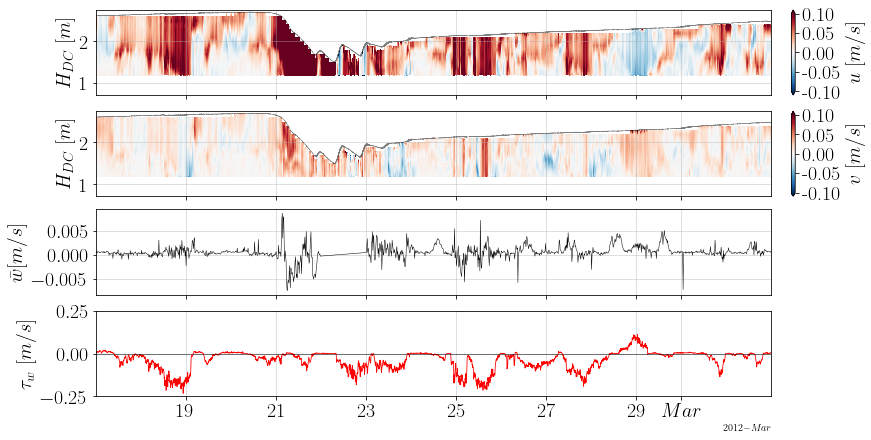
\includegraphics[width=\textwidth]{Imagenes/vels.png}
        \caption{Time-series of: $u$ and $v$ in the vertical, averaged vertical velocity, and wind stress.}
        \label{fig:vels}
    \end{figure}
    
    The observed dynamic of the upper velocity at the window shown in Fig. \ref{fig:vels} is such that when wind stress has positive velocity, considering positive the direction of the streamflow, the along-estuary water velocity is negative and vice versa. The magnitude of wind stress does not change this behavior along time, but as the water level increase, the estuarine velocity gets smaller for the same wind-stress magnitude. However, when wind stress is very small the dynamic change, and the upper along-estuary velocity at the window goes in the same direction as the wind stress at the surface. \\
    
    For the average vertical velocity in the water column ($\hat{w}$) (Fig. \ref{fig:vels}) we can observe mainly positive values (upwards), but there is no interesting behavior in it until the second period when we observed more changes, other than small fluctuations during a wind event. We could observe important peaks when the wind was starting to blow and, in some cases, right after the wind finished, showing that layers are going upwards at that moment. Also, we observed negative values during the first wind event on the second period, showing probably that the surface tilt is returning to its initial state.\\
    
    To observe in detail the behavior of the water column, densities and velocity profiles for each sensor were plotted in certain instants in the first wind event of the second period (Fig. \ref{fig:perfiles2}). This wind event is characterized by two wind increases and a period in the middle with small wind stress that lasted 3 hours approximately. The profiles before the event, during the first increase, the middle period, the second increase, and after the event were plotted.\\

    \newpage

    \begin{figure}[h!]
      \centering
      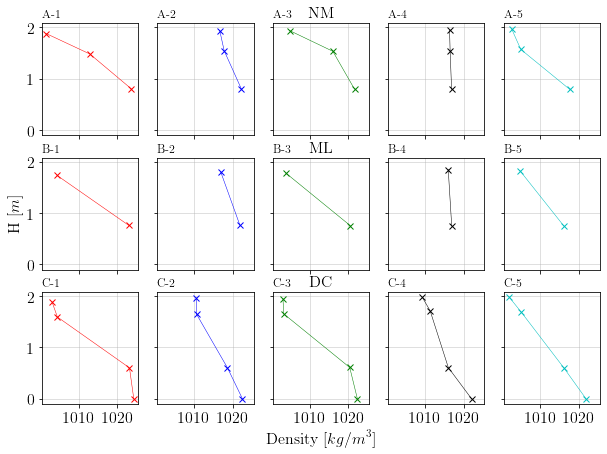
\includegraphics[width=0.85\textwidth]{Imagenes/perf.png}
      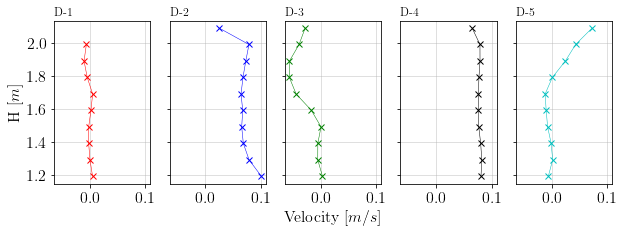
\includegraphics[width=0.85\textwidth]{Imagenes/vel.png}
      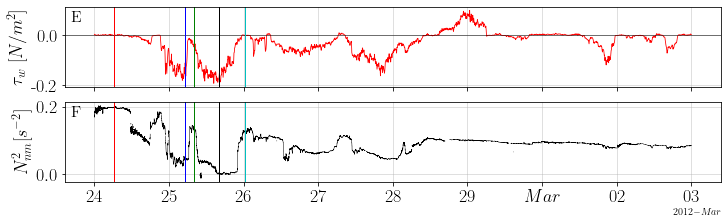
\includegraphics[width=0.85\textwidth]{Imagenes/n2.png}
      \caption{Density profiles at locations (A) NM, (B) ML and (C) DC, and (D) velocity profiles of 5 moments before, during, and after a full upwelling event, and time-series of (E) wind stress and (F) buoyancy frequency showing the plotted instants.}
      \label{fig:perfiles2}
    \end{figure}

    \newpage
    
    We could notice that before the wind event the water column is stratified, and the velocity is zero. During the first part of the event, the principal effect is the density increase near the surface and the positive velocity in all the visible part of the water column. Then, when the wind stopped the estuary went stratified with similar values of density to the first profiles, but the velocity had a different behavior, and went negative in the upper layer, probably showing that the water is returning to its original state or that when wind stress is too small the surface water that goes into the same direction of the wind gets thicker and starts to be detected by the ADCP. When the wind reaches its maximum the water column is less stratified than in the first increase and velocity has bigger values. Finally, the last profiles show positive velocities at the surface and as there is no wind at that moment, maybe is showing the freshwater passing throw the estuary, also, the density profiles show a stratified estuary but less than before the event, meaning there was mixing in the water column during the wind event.\\
    
    When the wind is blowing inland, shear stress causes a set up at the end of the estuary by driving water away from the free surface, increasing upstream hydrostatic pressure and causing estuarine recirculation. This causes the pycnocline to move towards the surface and increase in density where the surface layer used to be. This is what is happening in Fig. \ref{fig:perfiles2}, where NM has been affected first and more abruptly than ML and DC, the latter being the one that changes its density the least. This may be because NM is the closest sensor to the mouth of the estuary, and therefore it is the one that detects the pycnocline first, followed by ML and DC.\\
    
    On the other hand, buoyancy frequency values when wind stress is zero decreased, going from 0.2 to 0.1 $kg/m^3$  showing less stratification after the big wind event. Also, we can notice that $N^2$ is steadier after the wind event and decrease less for winds of the same magnitude (Fig. \ref{fig:perfiles2}).\\

    In Fig. \ref{fig:surf2} there is a closer look of the surface fluctuations behavior. First, in the wavelet analysis we observed three events of wave overtopping, which show a concentration of frequencies in the range from $2*10^{-2}$ to $2*10^{-1}$ Hz. Also, we observed that during the wind event the frequencies showed less concentration than in the wave overtopping event and was observed in the range of frequencies between $10^{-2}$ and $2*10^{-1}$ Hz. Second, the standardized height ($\hat{H}$) showed an increase with a positive peak when the wind started blowing, which when it went stronger decreased to negative values with lots of surface fluctuations. When the wind stopped the height return to positive values near 0. This is indicating an inclination of the surface or a set up. \\

    \begin{figure}[h!]
      \centering
      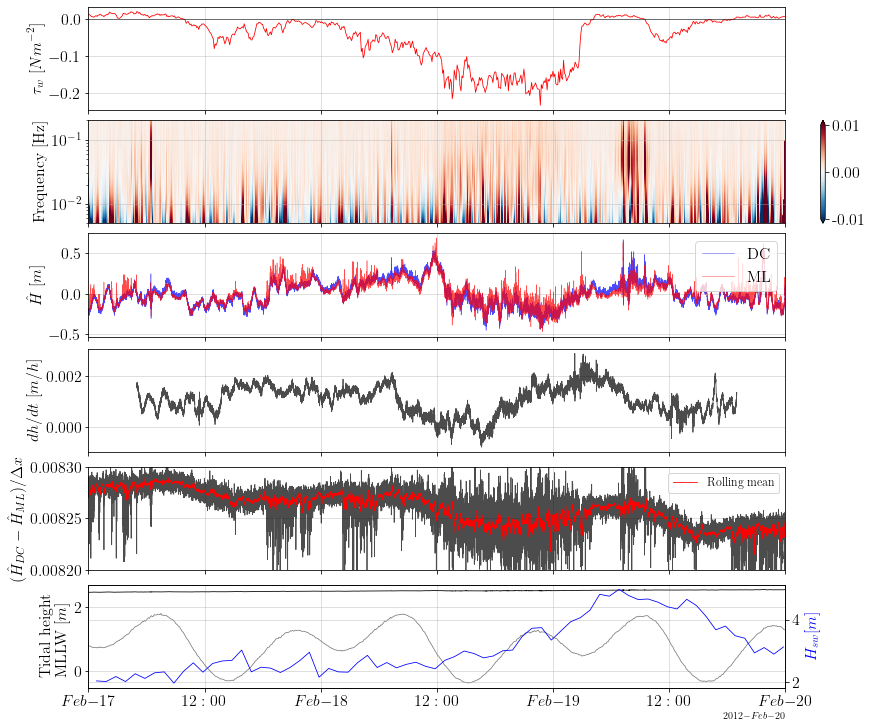
\includegraphics[width=0.9\textwidth]{Imagenes/surf2.png}
      \caption{Time-series of wind stress ($\tau_w$), depth wavelet frequency analysis at DC, standardized depth ($\hat{H}$) in DC and ML locations, the change of the water level in a 2-hour frame ($dh/dt$), standardized depth change between locations DC and ML ($(\hat{H}_{DC}-\hat{H}_{ML})/\Delta x$) with its rolling mean, and significant wave height in Halfmoon Bay (blue), Pescadero estuary water level (black) and tidal height in San Francisco (gray) in MLLW datum.}
      \label{fig:surf2}
    \end{figure}
    
    The change of the depth in time showed mainly positive values almost all the period (Fig. \ref{fig:surf2}), meaning that the water level is increasing most of the time. The only moment when the change was negative for more than an hour occur at the beginning of the wind event. Also, at the end of the time series there is a peak of negative values with unknown cause. The difference between the standardized height of DC and ML along-estuary indicates that when this value increases, the height in ML is smaller and the height in DC is larger, and vice versa. This could be caused by both the wind and other external factors such as inflow from upstream, flow that may be entering or escaping through the sand bar, among others. In Fig. \ref{fig:surf2} at the beginning of the time series the values of $\Delta \hat{H}/\Delta x$ are oscillating slightly around 0 with a wavelength of 24 h approximately. When the wind started blowing, the values turned negative, showing that DC decreased more than ML. After the wind event, the values continued the oscillations, but with more amplitude than before.\\
    
    The spectral analysis of the depth in DC, ML and NM shows that between frequencies of $4*10^{-3}$ and $1*10^{-2}$ Hz, around a period of 2 min, there is an increase in Power Spectral Density (PSD) (Fig. \ref{fig:freq}), showing us the presence of infragravity waves in Pescadero. If we add to the spectral analysis the wind stress and compare it we observed some similarities in the frequencies. Between $8*10^{-5}$ and $1*10^{-4}$ Hz there is an increase in PSD for wind and depth at NM, that is for the period around 200 min, and also between $1*10^{-4}$ and $1.1*10^{-4}$ Hz we notice peaks in wind and depth in ML and DC, that correspond to 140 min approximately. In addition we observed two peaks in wind stress between $2*10^{-5}$ and $5*10^{-5}$ Hz, that is between 700 and 300 min, while in the depth spectrum we observed some increases in the three sites for the same range but with less significance.
    
    \begin{figure}[h!]
      \centering
      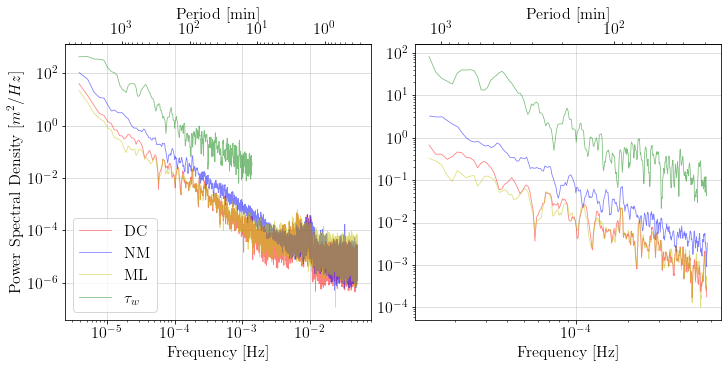
\includegraphics[width=0.9\textwidth]{Imagenes/freqs.png}
      \caption{Frequency spectra of water level fluctuations in the estuary at sites in NM, DC and ML, and of wind surface stress between 11 Feb. and 20 Feb. with a close up of the lower frequencies.}
      \label{fig:freq}
    \end{figure}




\end{document}